\documentclass{article}

% Language setting
% Replace `english' with e.g. `spanish' to change the document language
\usepackage[english]{babel}

% Set page size and margins
% Replace `letterpaper' with`a4paper' for UK/EU standard size
\usepackage[letterpaper,top=2cm,bottom=2cm,left=3cm,right=3cm,marginparwidth=1.75cm]{geometry}

% Useful packages
\usepackage{amsmath}
\usepackage{graphicx}
\usepackage[colorlinks=true, allcolors=blue]{hyperref}

\title{Cash-flow maturity and risk premia in CDS markets.}
\author{Antonio Pineda, Nidhi Beeravolu, Kausthub Keshava and Diana Castellanos}

\begin{document}
\maketitle

\begin{Data science tools for finance final project}
Professor: Jeremy Bejerano.
\end{abstract}

\section{Introduction}

The present project is an academic exercise designed to replicate and analyze the Credit Default Swap (CDS) returns specified by \cite{kelly2017}. The dataset, sourced from the repositories of Markit on Wharthon Research Data Services (WRDS), provides the data foundation upon which our replication model is constructed. \\

This work is designed to not only corroborate the meticulous work of \cite{kelly2017} but also to substantiate the theoretical implications proposed by \cite{Palhares2013} concerning the maturation of cash-flows and their correlation with the risk premia observed in the market for credit default swaps.\\

The paper is structured as follows. Section 2 introduces the model of CDS returns, detailing the theoretical framework and the mathematical underpinnings that guide the analysis. Section 3 provides a description of the data sourced from Markit and presents summary statistics to offer insights into the dataset's characteristics and the underlying market dynamics. Section 4 delves into the estimated CDS returns, employing the proposed model to analyze the dataset and interpret the results. The findings reveal that [WRITE RESULTS], highlighting the implications of [WRITE KEY VARIABLES] on CDS returns.  In conclusion, the paper demonstrates [WRITE MAIN CONCLUSION].


\section{Credit default swap returns definition.}

According to  \cite{Palhares2013}, CDS returns are definite as:

\begin{equation}
    CDS_{t}^{ret} = \frac{CDS_{t-1}}{250} + \Delta CDS_{t} \times RD_{t-1}.

\end{equation}

The right-hand side of the equation is composed of two parts: the carry component and the capital gain return. \

The carry component reflects the return accrued from the seller’s receipt of insurance premium payments. The second term represents the capital gain return, which is calculated by multiplying the change in the credit default swap (CDS) spread by the lagged risky duration of the contract, denoted as \( RD_{t-1} \). This risky duration adjusts the future CDS spread received by the seller to its present value. When this value is multiplied by the change in spread, it estimates the logarithmic capital gain for the seller who is in a short position.\\

The risky duration for CDS of maturity $M$ years with quarterly premium payments is computed as


\begin{equation}
RD_t = \frac{1}{4} \sum_{j=1}^{4M} e^{-\frac{j\lambda}{4}} \cdot e^{-\frac{j(r_{\frac{j}{4}, t})}{4}},
\end{equation}


where:

$e^{-\frac{j\lambda}{4}}$ is the quarterly survival probability, \ 

$r^{\frac{j}{4}}_t$ is the risk-free rate for the quarter $\frac{j}{4}$,\

and $e^{-j\frac{j(r^{\frac{j}{4}})}_{4}}$ is the quarterly discount function. And  $\lambda$ each day from the 5-year spread as

\[
\lambda = 4 \log \left(1 + \frac{\text{CDS}}{4L}\right),
\]

where $\text{CDS}$ is the spread and $L$ is the loss given default (assumed to be 60\%). The risk-free term structure is constructed using swap rates for maturities 3 and 6 months and US Treasury yields for maturities from 1 year to 10 years.


\section{Data.}

\section{Results.}

\subsection{Definition}

Simply use the section and subsection commands, as in this example document! With Overleaf, all the formatting and numbering is handled automatically according to the template you've chosen. If you're using Rich Text mode, you can also create new section and subsections via the buttons in the editor toolbar.

\subsection{How to include Figures}

First you have to upload the image file from your computer using the upload link in the file-tree menu. Then use the includegraphics command to include it in your document. Use the figure environment and the caption command to add a number and a caption to your figure. See the code for Figure \ref{fig:myplot} in this section for an example.

Note that your figure will automatically be placed in the most appropriate place for it, given the surrounding text and taking into account other figures or tables that may be close by. You can find out more about adding images to your documents in this help article on \href{https://www.overleaf.com/learn/how-to/Including_images_on_Overleaf}{including images on Overleaf}.

\begin{figure}
\centering
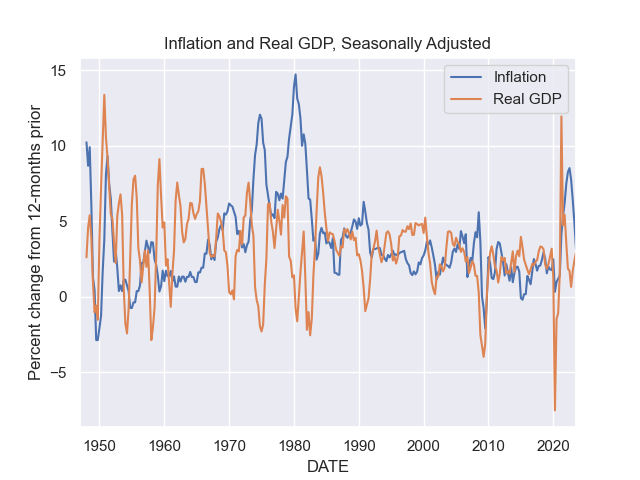
\includegraphics[width=0.75\textwidth]{../output/example_plot.png}
\caption{\label{fig:myplot}This image was uploaded via the file-tree menu.}
\end{figure}


\subsection{How to add Comments and Track Changes}

Comments can be added to your project by highlighting some text and clicking ``Add comment'' in the top right of the editor pane. To view existing comments, click on the Review menu in the toolbar above. To reply to a comment, click on the Reply button in the lower right corner of the comment. You can close the Review pane by clicking its name on the toolbar when you're done reviewing for the time being.

Track changes are available on all our \href{https://www.overleaf.com/user/subscription/plans}{premium plans}, and can be toggled on or off using the option at the top of the Review pane. Track changes allow you to keep track of every change made to the document, along with the person making the change. 

\subsection{How to add Lists}

You can make lists with automatic numbering \dots

\begin{enumerate}
\item Like this,
\item and like this.
\end{enumerate}
\dots or bullet points \dots
\begin{itemize}
\item Like this,
\item and like this.
\end{itemize}

\subsection{How to write Mathematics}

\LaTeX{} is great at typesetting mathematics. Let $X_1, X_2, \ldots, X_n$ be a sequence of independent and identically distributed random variables with $\text{E}[X_i] = \mu$ and $\text{Var}[X_i] = \sigma^2 < \infty$, and let
\[S_n = \frac{X_1 + X_2 + \cdots + X_n}{n}
      = \frac{1}{n}\sum_{i}^{n} X_i\]
denote their mean. Then as $n$ approaches infinity, the random variables $\sqrt{n}(S_n - \mu)$ converge in distribution to a normal $\mathcal{N}(0, \sigma^2)$.


\subsection{How to change the margins and paper size}

Usually the template you're using will have the page margins and paper size set correctly for that use-case. For example, if you're using a journal article template provided by the journal publisher, that template will be formatted according to their requirements. In these cases, it's best not to alter the margins directly.

If however you're using a more general template, such as this one, and would like to alter the margins, a common way to do so is via the geometry package. You can find the geometry package loaded in the preamble at the top of this example file, and if you'd like to learn more about how to adjust the settings, please visit this help article on \href{https://www.overleaf.com/learn/latex/page_size_and_margins}{page size and margins}.

\subsection{How to change the document language and spell check settings}

Overleaf supports many different languages, including multiple different languages within one document. 

To configure the document language, simply edit the option provided to the babel package in the preamble at the top of this example project. To learn more about the different options, please visit this help article on \href{https://www.overleaf.com/learn/latex/International_language_support}{international language support}.

To change the spell check language, simply open the Overleaf menu at the top left of the editor window, scroll down to the spell check setting, and adjust accordingly.

\subsection{How to add Citations and a References List}

You can simply upload a \verb|.bib| file containing your BibTeX entries, created with a tool such as JabRef. 
You can then cite entries from it, like this: 
\cite{fama1992cross} or \cite{sharpe1964capital}. 
Just remember to specify a bibliography style, as well as the filename of the \verb|.bib|. You can find a \href{https://www.overleaf.com/help/97-how-to-include-a-bibliography-using-bibtex}{video tutorial here} to learn more about BibTeX.

If you have an \href{https://www.overleaf.com/user/subscription/plans}{upgraded account}, you can also import your Mendeley or Zotero library directly as a \verb|.bib| file, via the upload menu in the file-tree.

\subsection{Good luck!}

We hope you find Overleaf useful, and do take a look at our \href{https://www.overleaf.com/learn}{help library} for more tutorials and user guides! Please also let us know if you have any feedback using the Contact Us link at the bottom of the Overleaf menu --- or use the contact form at \url{https://www.overleaf.com/contact}.

\bibliographystyle{alpha}
\bibliography{bibliography}

\end{document}